% \subsection{Kiến trúc hệ thống}
% \subsubsection{Đặc trưng của hệ thống}

% Hệ thống có những \textbf{đặc điểm kỹ thuật và nghiệp vụ} sau đây, ảnh hưởng trực tiếp đến việc chọn kiến trúc:

% \begin{longtable}{|>{\raggedright\arraybackslash}p{5cm}|>{\raggedright\arraybackslash}p{10cm}|}
% \hline
% \textbf{Nhóm đặc trưng} & \textbf{Mô tả chi tiết} \\
% \hline
% \endfirsthead

% \hline
% \textbf{Nhóm đặc trưng} & \textbf{Mô tả chi tiết} \\
% \hline
% \endhead

% \hline
% \endfoot

% 1. Nhiều loại người dùng & Hệ thống phục vụ 3 vai trò: người thuê, người chia sẻ (chủ xe), và admin. Cả 2 vai trò chính (renter/owner) đều có thể là cùng 1 người dùng. \\
% \hline
% 2. Giao tiếp thời gian thực nhẹ & Ứng dụng cần cập nhật \textbf{vị trí xe}, \textbf{tình trạng pin}, và \textbf{trạng thái thuê xe} theo thời gian gần thực (real-time-ish) nhưng không yêu cầu tốc độ quá cao như game hay trading. \\
% \hline
% 3. Dữ liệu không đồng bộ & Xe có thể được thêm, xóa, cập nhật vị trí, trạng thái thuê... thường xuyên. \\
% \hline
% 4. Hỗ trợ di động và web & Người dùng có thể thao tác qua \textbf{ứng dụng di động} (React Native) hoặc \textbf{trang web} (React.js). \\
% \hline
% 5. Khối lượng truy cập phân tán, có thể tăng dần & Hệ thống hướng đến cộng đồng dân cư / trường học, sau đó có thể mở rộng ra quy mô thành phố. Cần dễ mở rộng (scalable). \\
% \hline
% 6. Có mô-đun AI tích hợp & Module dự đoán thời gian thuê hiệu quả (ML) chạy độc lập hoặc song song với backend chính. \\
% \hline
% 7. Có yếu tố học thuật P2P & Mô phỏng cơ chế chia sẻ ngang hàng: người dùng vừa thuê vừa cho thuê, có cơ chế đánh giá uy tín (trust score). \\
% \hline
% 8. Cần bảo mật và xác thực & Dữ liệu người dùng, vị trí và giao dịch phải được bảo vệ bằng cơ chế xác thực và mã hóa. \\
% \hline
% 9. Tính mở rộng công nghệ & Dễ tích hợp thêm IoT (nếu gắn cảm biến pin xe), thanh toán điện tử, hoặc AI nâng cao sau này. \\
% \hline
% \end{longtable}

% \subsubsection*{Phân tích yêu cầu kỹ thuật (non-functional requirements)}

% \begin{longtable}{|>{\raggedright\arraybackslash}p{4cm}|>{\raggedright\arraybackslash}p{4cm}|>{\raggedright\arraybackslash}p{7cm}|}
% \hline
% \textbf{Tiêu chí} & \textbf{Mức yêu cầu} & \textbf{Ý nghĩa} \\
% \hline
% \endfirsthead

% \hline
% \textbf{Tiêu chí} & \textbf{Mức yêu cầu} & \textbf{Ý nghĩa} \\
% \hline
% \endhead

% \hline
% \endfoot

% Hiệu năng & Trung bình → Cao & Phản hồi trong $\leq$ 2s cho các thao tác chính (tìm xe, thuê xe). \\
% \hline
% Scalability (mở rộng) & Quan trọng & Có thể mở rộng khi số người thuê tăng nhanh. \\
% \hline
% Availability (sẵn sàng) & Trung bình & Không yêu cầu 24/7 nhưng phải ổn định khi sử dụng. \\
% \hline
% Maintainability (dễ bảo trì) & Cao & Kiến trúc module tách biệt, dễ nâng cấp. \\
% \hline
% Security (bảo mật) & Quan trọng & Xác thực người dùng, mã hóa JWT, ẩn vị trí chính xác của chủ xe. \\
% \hline
% Interoperability (tích hợp) & Quan trọng & Dễ tích hợp AI module, API bản đồ, thanh toán. \\
% \hline
% \end{longtable}

% \subsubsection{Các Architectural Styles phổ biến}
% \begin{longtable}{|>{\raggedright\arraybackslash}p{3cm}|>{\raggedright\arraybackslash}p{4cm}|>{\raggedright\arraybackslash}p{3.5cm}|>{\raggedright\arraybackslash}p{3.5cm}|}
% \hline
% \textbf{Style} & \textbf{Mô tả} & \textbf{Ưu điểm} & \textbf{Nhược điểm} \\
% \hline
% \endfirsthead
% \hline
% \textbf{Style} & \textbf{Mô tả} & \textbf{Ưu điểm} & \textbf{Nhược điểm} \\
% \hline
% \endhead
% \hline
% \endfoot
% Layered & Chia thành các tầng: Presentation, Application, Domain, Infrastructure. Mỗi tầng chỉ giao tiếp với tầng liền kề. & Dễ bảo trì và mở rộng. \newline Thay đổi một tầng không ảnh hưởng tầng khác. & Phức tạp khi có nhiều tầng. \newline Dễ rò rỉ logic giữa các tầng. \\
% \hline
% Monolithic & Toàn bộ ứng dụng (UI, logic, DB) trong một package duy nhất. & Đơn giản, dễ phát triển và deploy. \newline Phù hợp dự án nhỏ/MVP. & Khó scale. \newline Deploy một phần phải restart toàn bộ. \newline Logic chồng chéo. \\
% \hline
% Microservices & Chia ứng dụng thành các service độc lập, giao tiếp qua API/message queue. & Scale riêng từng service. \newline Chịu lỗi tốt. \newline Hỗ trợ CI/CD. & Hạ tầng phức tạp (Gateway, orchestration). \newline Debug khó. \newline Chi phí cao. \\
% \hline
% Event-driven & Các module giao tiếp qua sự kiện (event bus/pub-sub). & Tốt cho real-time và async. \newline Dễ mở rộng module mới. & Thiết kế phức tạp. \newline Cần message broker (Kafka, RabbitMQ). \\
% \hline
% Microkernel (Plugin) & Core system nhỏ + các plugin mở rộng chức năng. & Dễ thêm module mới. \newline Core gọn, dễ bảo trì. & Quản lý interface phức tạp. \newline Ít framework hỗ trợ. \\
% \hline
% Serverless / FaaS & Chạy các hàm độc lập trên cloud (AWS Lambda, Firebase Functions). & Không quản lý server. \newline Tự động scale. & Quản lý state khó. \newline Cold start delay. \newline Chi phí cao khi scale lớn. \\
% \hline
% \end{longtable}

% \subsubsection*{Tổng kết mức độ phù hợp với hệ thống chia sẻ xe máy điện P2P}
% \begin{longtable}{|>{\raggedright\arraybackslash}p{2.5cm}|>{\centering\arraybackslash}p{2.2cm}|>{\raggedright\arraybackslash}p{9.5cm}|}
% \hline
% \textbf{Style} & \textbf{Mức độ} & \textbf{Vai trò / Lý do} \\
% \hline
% \endfirsthead

% \hline
% \textbf{Style} & \textbf{Mức độ} & \textbf{Vai trò / Lý do} \\
% \hline
% \endhead

% \hline
% \endfoot
% Layered & \textbf{Rất cao} ⭐⭐⭐⭐☆ & \textbf{Style chính} cho toàn hệ thống. Nhiều module (user, xe, AI, P2P) cần tách tầng rõ ràng để dễ quản lý, bảo trì và mở rộng. \\
% \hline

% Event-driven & \textbf{Cao} ⭐⭐⭐☆☆ & \textbf{Cơ chế giao tiếp bổ sung}. Phù hợp real-time (vị trí xe, trạng thái thuê), AI training (học từ event), P2P sync, notification. \\
% \hline

% Microkernel & Trung bình ⭐⭐☆☆☆ & Ý tưởng plugin (AI, Payment) tốt cho \textbf{mở rộng module} sau này, nhưng không cần triển khai riêng trong đồ án. \\
% \hline

% Microservices & Trung bình ⭐⭐☆☆☆ & Ý tưởng tách module (P2P, AI, Payment) phù hợp, nhưng \textbf{setup phức tạp}, quá nặng cho quy mô đồ án. Có thể mô phỏng bằng Clean Architecture. \\
% \hline

% Monolithic & Thấp ⭐☆☆☆☆ & \textbf{Không phù hợp}. Hệ thống cần mở rộng nhiều module (AI, P2P, payment) nên kiến trúc nguyên khối sẽ cồng kềnh, khó bảo trì. \\
% \hline

% Serverless & Thấp ⭐☆☆☆☆ & Chỉ phù hợp \textbf{tác vụ nhỏ lẻ} (AI inference, notification). Toàn hệ thống cần quản lý state (rental, payment, peer state) nên không nên dùng serverless. \\
% \hline
% \end{longtable}

% \subsubsection{Layered Architecture}
% Tuy nhiên trong phạm vi Layered Architecture, có nhiều pattern triển khai như 3-Tier, MVC, hay Clean Architecture. Để đánh giá kiến trúc phù hợp nhất với đề tài, cần có so sánh chi tiết giữa các Architecture pattern này.

% % \begin{longtable}{|>{\raggedright\arraybackslash}p{3cm}|>{\raggedright\arraybackslash}p{4cm}|>{\raggedright\arraybackslash}p{4cm}|>{\raggedright\arraybackslash}p{3.5cm}|}
% % \hline
% % \textbf{Tiêu chí} & \textbf{Layered Architecture} & \textbf{Clean Architecture} & \textbf{Điểm khác biệt} \\
% % \hline
% % \endfirsthead

% % \hline
% % \textbf{Tiêu chí} & \textbf{Layered Architecture} & \textbf{Clean Architecture} & \textbf{Điểm khác biệt} \\
% % \hline
% % \endhead

% % \hline
% % \endfoot

% % Mục tiêu & Tách hệ thống thành các tầng logic (UI, Business, Data) để dễ bảo trì, mở rộng. & Đảm bảo hướng phụ thuộc luôn đi từ ngoài vào trong (về phía core business). & Clean Architecture \textbf{kế thừa} Layered Architecture, nhưng \textbf{thêm nguyên tắc phụ thuộc ngược}. \\
% % \hline
% % Cách chia tầng & Theo \textbf{chức năng kỹ thuật (technical layers)}: UI → Service → Repository → DB. & Theo \textbf{miền nghiệp vụ (domain layers)}: Entities → Use Cases → Interface Adapters → Frameworks. & Clean Architecture là \textbf{phiên bản tiến hóa} của Layered, tập trung vào domain thay vì kỹ thuật. \\
% % \hline
% % Hướng phụ thuộc & Phụ thuộc \textbf{xuôi} (UI gọi xuống Service, Service gọi xuống Repository). & Phụ thuộc \textbf{ngược} (Infrastructure phụ thuộc vào Use Cases, chứ không ngược lại). & Đây là điểm khác biệt \textbf{cốt lõi nhất}. \\
% % \hline
% % Đối tượng trung tâm & Dữ liệu / logic kỹ thuật. & Domain (business rules). & Clean chuyển "tâm" của hệ thống về \textbf{use case và entity}. \\
% % \hline
% % Testability & Khó test độc lập vì các tầng kỹ thuật phụ thuộc trực tiếp vào nhau. & Dễ test unit vì core tách rời hạ tầng (framework, DB, UI). & Clean giải quyết nhược điểm của Layered. \\
% % \hline
% % \end{longtable}

% % \begin{figure}[H]
% %     \centering
% %     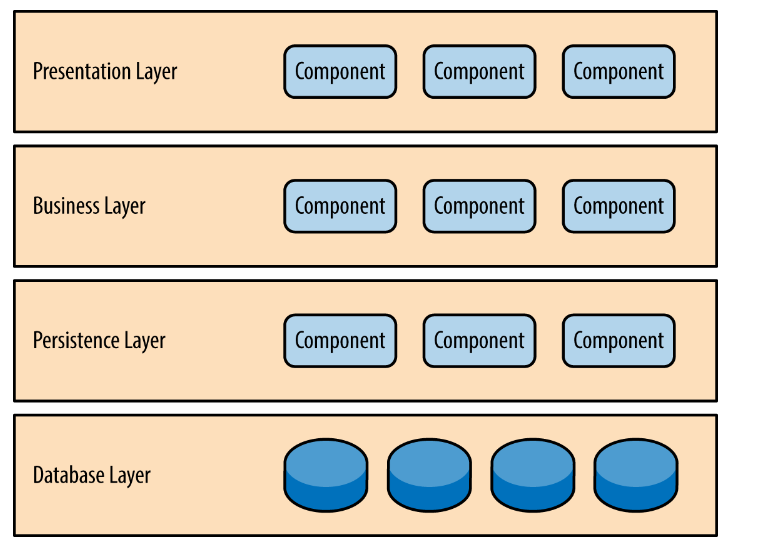
\includegraphics[width=0.7\textwidth]{Images/Arch/layer.png}
% %     \caption{Layered Architecture}
% %     \label{fig:layered-arch}
% % \end{figure}

% % \subsubsubsection*{So sánh các Architecture Pattern phổ biến trong Layer Architecture Style vs Clean Architecture}

% % \begin{longtable}{|>{\raggedright\arraybackslash}p{6.5cm}|>{\raggedright\arraybackslash}p{2.5cm}|>{\raggedright\arraybackslash}p{2.5cm}|>{\raggedright\arraybackslash}p{3cm}|}
% % \hline
% % \textbf{Tiêu chí} & \textbf{3-Tier} & \textbf{MVC} & \textbf{Clean Architecture} \\
% % \hline
% % \endfirsthead

% % \hline
% % \textbf{Tiêu chí} & \textbf{3-Tier} & \textbf{MVC} & \textbf{Clean Architecture} \\
% % \hline
% % \endhead

% % \hline
% % \endfoot

% % Tách biệt business logic khỏi infra & Trung bình & Trung bình & Cao \\
% % \hline
% % Testability & Trung bình & Trung bình & Cao \\
% % \hline
% % Dễ triển khai MVP & Cao & Cao & Trung bình \\
% % \hline
% % Tích hợp AI/externals & Trung bình & Trung bình & Cao \\
% % \hline
% % Handling real-time / event & Trung bình & Trung bình & Cao\\
% % \hline
% % \end{longtable}
% % Dựa trên những phân tích trên, hệ thống chia sẻ xe máy điện P2P sẽ sử dụng \textbf{Clean Architecture} làm kiến trúc chính, kết hợp với \textbf{Event-driven Architecture} để xử lý các tác vụ bất đồng bộ và real-time. Cụ thể:
% % \begin{itemize}
% % \item \textbf{Clean Architecture}: Cung cấp cấu trúc tổng thể cho hệ thống, đảm bảo tính module hóa, dễ bảo trì và mở rộng.
% % \item \textbf{Event-driven Architecture}: Được tích hợp như một cơ chế giao tiếp bổ sung giữa các module, đặc biệt phục vụ cho việc đồng bộ trạng thái xe, gửi thông báo real-time, và cung cấp dữ liệu cho module AI/ML.
% % \item \textbf{Client-Server}: Là nền tảng giao tiếp cơ bản giữa frontend (mobile/web) và backend thông qua RESTful API.
% % \end{itemize}

% % \begin{figure}[H]
% %     \centering
% %     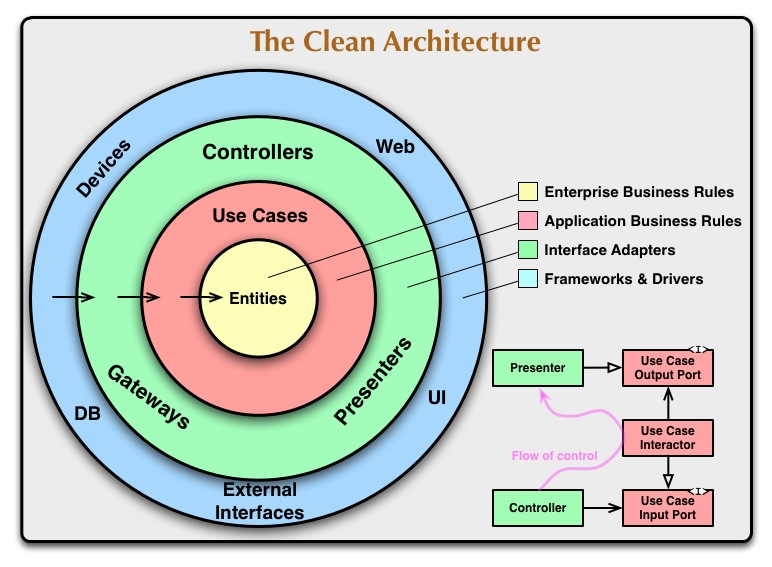
\includegraphics[width=0.7\textwidth]{Images/Arch/clean.png}
% %     \caption{Clean Architecture (Uncle Bob)}
% %     \label{fig:clean-arch}
% % \end{figure}

% \subsubsection*{a. MVC (Model -- View -- Controller)}
% Mô hình MVC được giới thiệu lần đầu bởi Trygve Reenskaug vào những năm 1970, nhằm tách biệt rõ ba phần chính trong ứng dụng: dữ liệu (Model), giao diện (View), và điều khiển (Controller).
% \begin{figure}[h]
% \centering
% 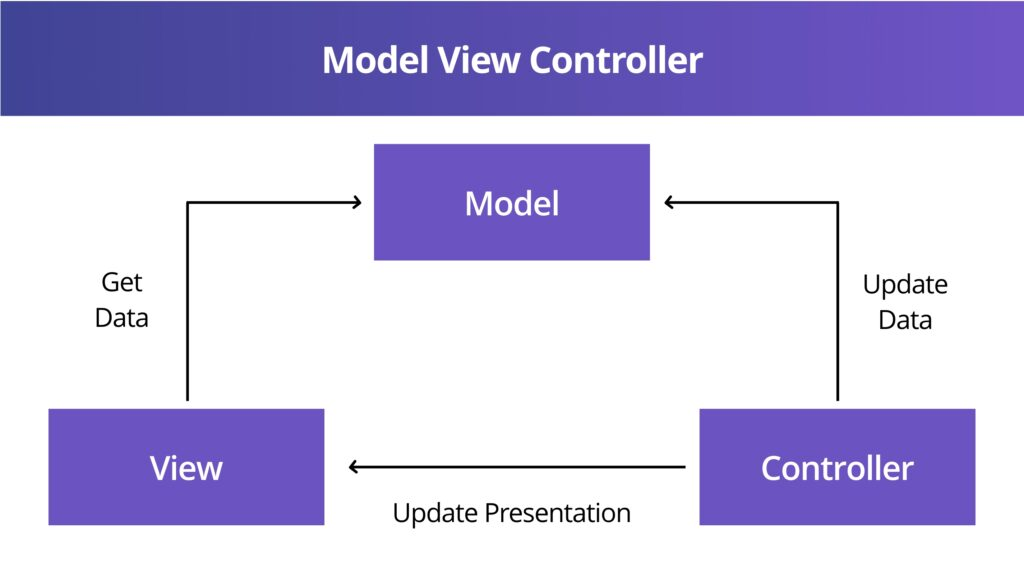
\includegraphics[height=0.3\textheight,keepaspectratio]{Images/Arch/mvc.png}
% \caption{MVC Architectural Design Pattern}
% \label{fig:mvc}
% \end{figure}

% \begin{table}[h]
% \centering
% \begin{tabular}{>{\bfseries}p{3cm}p{10cm}}
% \toprule
% \textbf{Thành phần} & \textbf{Vai trò} \\
% \midrule
% Model & Quản lý dữ liệu và logic nghiệp vụ của ứng dụng. Model nhận yêu cầu từ Controller, xử lý và trả dữ liệu lại. \\
% \addlinespace
% View & Chịu trách nhiệm hiển thị dữ liệu của Model ra giao diện, không chứa logic nghiệp vụ. \\
% \addlinespace
% Controller & Xử lý thao tác từ người dùng (user input), thực hiện xác thực (nếu cần), gọi Model để thay đổi dữ liệu, sau đó cập nhật lại View. \\
% \bottomrule
% \end{tabular}
% \end{table}
% % Người dùng tương tác với giao diện (View). Controller nhận sự kiện, gọi Model để xử lý dữ liệu. Model cập nhật dữ liệu và gửi lại kết quả cho View để hiển thị.

% \subsubsection*{Ưu điểm}
% - Tách biệt giữa dữ liệu, giao diện và điều khiển → dễ bảo trì.\\
% - Phù hợp với ứng dụng nhỏ, ít tầng logic.

% \subsubsection*{Nhược điểm}
% - Controller và View phụ thuộc chặt chẽ → thay đổi UI phải sửa Controller.\\
% - Model có thể bị truy cập trực tiếp bởi View, vi phạm nguyên tắc ``Separation of Concerns''.\\
% - Khó kiểm thử (unit test) vì Controller gắn liền với giao diện.\\



% \subsubsection*{b. MVP (Model -- View -- Presenter)}
% MVP được phát triển để khắc phục nhược điểm của MVC, bằng cách tách logic xử lý giao diện ra khỏi View, giúp dễ test và bảo trì hơn.
% \begin{figure}[h]
% \centering
% 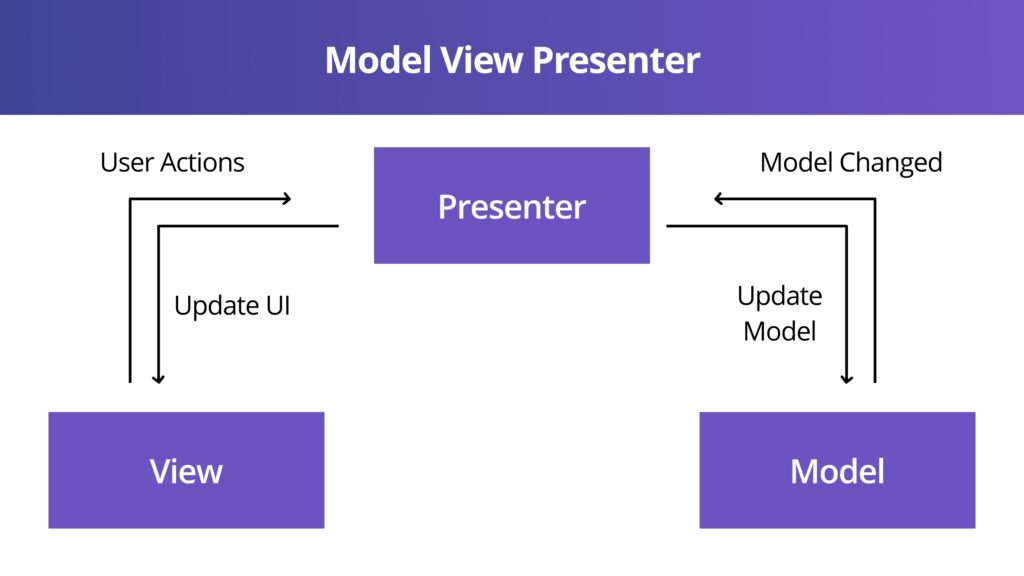
\includegraphics[height=0.3\textheight,keepaspectratio]{Images/Arch/mvp.png}
% \caption{MVP Architectural Design Pattern}
% \label{fig:mvp}
% \end{figure}

% \begin{table}[h]
% \centering
% \begin{tabular}{>{\bfseries}p{3cm}p{10cm}}
% \toprule
% \textbf{Thành phần} & \textbf{Vai trò} \\
% \midrule
% Model & Tập hợp các lớp mô tả logic nghiệp vụ và dữ liệu. Định nghĩa các quy tắc thao tác với dữ liệu. \\
% \addlinespace
% View & Hiển thị dữ liệu và chuyển tiếp sự kiện người dùng đến Presenter. Không chứa logic nghiệp vụ. \\
% \addlinespace
% Presenter & Trung gian giữa View và Model. Nhận input từ View, gọi Model xử lý, sau đó trả kết quả lại cho View để hiển thị. \\
% \bottomrule
% \end{tabular}
% \end{table}

% \subsubsection*{Ưu điểm}
% - View không biết Model tồn tại, chỉ nhận dữ liệu từ Presenter → tách biệt rõ ràng.\\
% - Dễ viết unit test cho Presenter vì không phụ thuộc vào UI framework.\\
% - Tăng khả năng tái sử dụng View và Model.

% \subsubsection*{Nhược điểm}
% - Presenter dễ trở thành ``God class'' nếu chứa quá nhiều logic.\\
% - Code nhiều hơn do phải tạo các interface giữa View $\leftrightarrow$ Presenter.\\
% - Quan hệ Presenter--View vẫn còn chặt (Presenter phải biết View để gọi update).

% \subsubsection*{c. MVVM (Model -- View -- ViewModel)}
% MVVM ra đời để loại bỏ sự phụ thuộc giữa Presenter và View trong MVP, bằng cách dùng cơ chế data binding hai chiều. Mô hình này được sử dụng phổ biến trong Android (Jetpack), iOS (SwiftUI) và Frontend (React, Vue, Angular).
% \begin{figure}[h]
% \centering
% 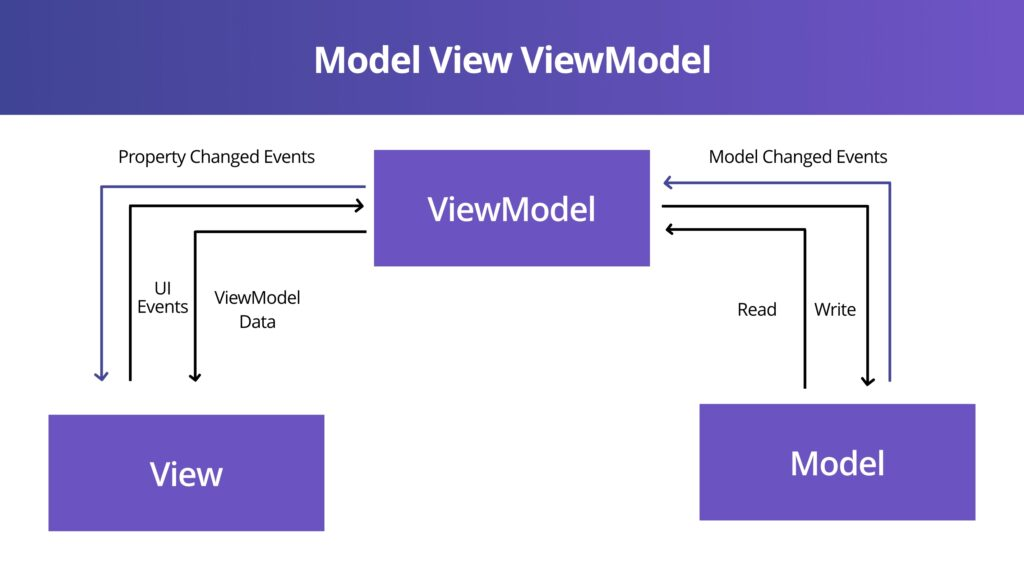
\includegraphics[height=0.3\textheight,keepaspectratio]{Images/Arch/mvvm.png}
% \caption{MVVM Architectural Design Pattern}
% \label{fig:mvvm}
% \end{figure}

% \begin{table}[h]
% \centering
% \begin{tabular}{>{\bfseries}p{3cm}p{10cm}}
% \toprule
% \textbf{Thành phần} & \textbf{Vai trò} \\
% \midrule
% Model & Lưu trữ dữ liệu và logic nghiệp vụ. Không giao tiếp trực tiếp với View. Expose dữ liệu qua các Observable/LiveData/Flow. \\
% \addlinespace
% View & Giao diện hiển thị dữ liệu, không chứa logic nghiệp vụ. Quan sát (observe) dữ liệu từ ViewModel và tự động cập nhật khi có thay đổi. \\
% \addlinespace
% ViewModel & Trung gian giữa Model và View. Gọi Model để lấy dữ liệu, xử lý và cung cấp data stream cho View. Sử dụng callback hoặc observable để cập nhật View. \\
% \bottomrule
% \end{tabular}
% \end{table}

% \subsubsection*{Ưu điểm}
% - View và ViewModel không biết nhau trực tiếp → giảm coupling.\\
% - Hỗ trợ binding tự động → code gọn, dễ bảo trì.\\
% - Dễ kiểm thử logic trong ViewModel.

% \subsubsection*{Nhược điểm}
% - Khó debug nếu có nhiều Observable phức tạp.\\
% - Dễ gây vòng lặp dữ liệu nếu binding hai chiều sai cách.\\
% - Yêu cầu hiểu biết về reactive programming.

% \subsubsection*{d. Clean Architecture}
% Clean Architecture được đề xuất bởi Robert C. Martin (Uncle Bob), nhằm chuẩn hóa cách tách biệt tầng trong ứng dụng -- đặc biệt cho các hệ thống lớn, dễ bảo trì, test và mở rộng. Kiến trúc này được chia thành các vòng (layers) đồng tâm, mọi phụ thuộc đều hướng vào trong.
% \begin{figure}[H]
%     \centering
%     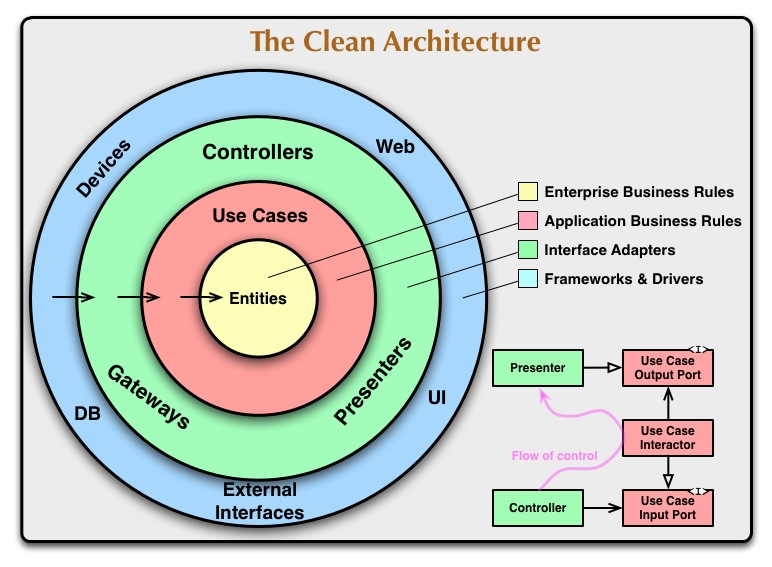
\includegraphics[width=0.9\textwidth]{Images/Arch/clean.png}
%     \caption{Clean Architecture (Uncle Bob)}
%     \label{fig:clean-arch}
% \end{figure}
% \textbf{Quy tắc phụ thuộc (Dependency Rule):} Tất cả phụ thuộc phải chỉ hướng vào trong -- nghĩa là lớp ngoài có thể gọi lớp trong, nhưng lớp trong không được biết gì về lớp ngoài.

% \newpage

% \subsubsection*{Các tầng chính}
% \begin{table}[h]
% \centering
% \begin{tabular}{>{\bfseries}p{4.5cm}p{4cm}p{4.5cm}}
% \toprule
% \textbf{Tầng} & \textbf{Thành phần chính} & \textbf{Vai trò} \\
% \midrule
% UI / Interface Layer & Controller, Presenter, ViewModel, View & Tiếp nhận và hiển thị dữ liệu với người dùng. \\
% \addlinespace
% Application Layer & UseCase Interactor, InputBoundary, OutputBoundary & Chứa logic nghiệp vụ ứng dụng (use case). \\
% \addlinespace
% Domain Layer & Entities & Chứa logic nghiệp vụ cốt lõi, không phụ thuộc framework. \\
% \addlinespace
% Infrastructure Layer & DataAccessInterface, DataAccess, Database & Thao tác lưu trữ dữ liệu (DB, API, file...). \\
% \bottomrule
% \end{tabular}
% \end{table}
% \subsubsection*{Luồng hoạt động chi tiết}
% \subsubsubsection*{Bước 1 -- Controller nhận input từ người dùng}
% \vspace{-0.3cm}
% Người dùng gửi request (qua web form, API, hay giao diện). Controller nhận dữ liệu đầu vào (Input Data) và gói lại trong một Data Transfer Object (DTO) -- ví dụ \texttt{CreateOrderRequest} hoặc \texttt{LoginRequest}. Controller không xử lý nghiệp vụ mà chuyển tiếp qua interface \texttt{InputBoundary}.
% \vspace{-0.7cm}
% \subsubsubsection*{Bước 2 -- InputBoundary chuyển dữ liệu vào Use Case}
% \vspace{-0.3cm}
% \texttt{InputBoundary} là một interface, đảm bảo Controller không phụ thuộc trực tiếp vào logic nghiệp vụ. \texttt{UseCaseInteractor} implement \texttt{InputBoundary}, nên khi Controller gọi interface này, luồng điều khiển vào bên trong Application Layer.
% \vspace{-0.5cm}
% \subsubsubsection*{Bước 3 -- Use Case Interactor thực thi nghiệp vụ}
% \vspace{-0.3cm}
% Đây là trái tim của ứng dụng (application business rules). \texttt{UseCaseInteractor}:\\
% - Gọi Entities để áp dụng logic nghiệp vụ (ví dụ: tính tổng tiền, kiểm tra điều kiện).\\
% - Dùng \texttt{DataAccessInterface} để lấy dữ liệu thật từ DB (thông qua repository).\\
% - Kết quả xử lý được đóng gói lại thành \texttt{OutputData} (cũng là POJO).
% \vspace{-0.5cm}
% \subsubsubsection*{Bước 4 -- OutputBoundary trả kết quả ra ngoài}
% \vspace{-0.3cm}
% Sau khi xử lý xong, \texttt{UseCaseInteractor} gửi \texttt{OutputData} qua \texttt{OutputBoundary} (interface). Presenter implement \texttt{OutputBoundary}, nên sẽ nhận được dữ liệu này.
% \vspace{-0.5cm}
% \subsubsubsection*{Bước 5 -- Presenter chuyển đổi dữ liệu cho UI}
% \vspace{-0.3cm}
% Presenter không xử lý nghiệp vụ mà chỉ lo định dạng dữ liệu để hiển thị:
% % \begin{itemize}[leftmargin=*]
% %     \item Chuyển Date thành chuỗi ``31/10/2025'', Currency thành ``1,000 VND''.
% %     \item Đưa các cờ (flags) như ``button enabled'', ``menu visible'' vào ViewModel.
% % \end{itemize}
% ViewModel là một Data Transfer Object (DTO) chứa dữ liệu UI-friendly.
% \vspace{-0.5cm}
% \subsubsubsection*{Bước 6 -- View hiển thị dữ liệu cho người dùng}
% \vspace{-0.3cm}
% View chỉ cần nhận ViewModel và render ra giao diện (HTML, React component, XML layout, ...). View không chứa logic nghiệp vụ, chỉ hiển thị đúng dữ liệu đã được Presenter chuẩn bị.
% \begin{figure}[h]
% \centering
% 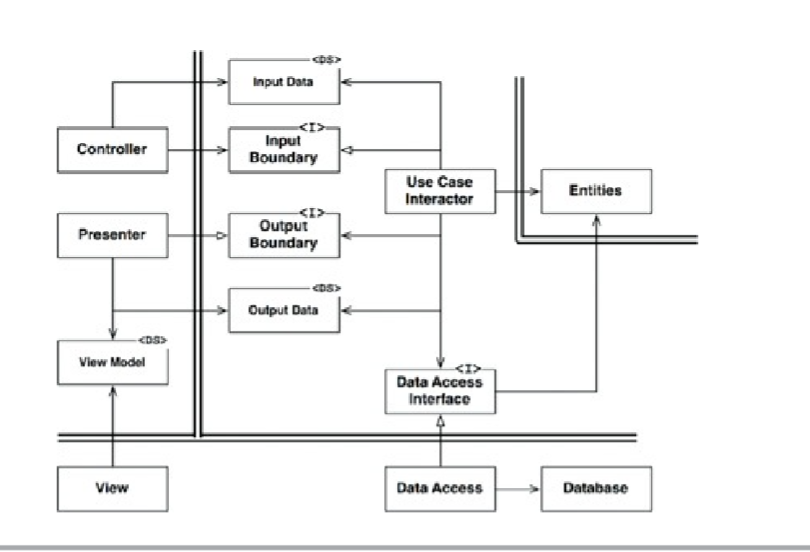
\includegraphics[height=0.5\textwidth]{Images/Arch/clean_flow.png}
% \caption{A typical scenario for a system utilizing a database follow Clean Architecture}
% \label{fig:clean_full}
% \end{figure}
% % \vspace{-0.5cm}
% % \subsubsection*{Ý nghĩa của thiết kế}
% % \begin{table}[h]
% % \centering
% % \begin{tabular}{>{\bfseries}p{5cm}p{8cm}}
% % \toprule
% % \textbf{Mục tiêu} & \textbf{Cách đạt được} \\
% % \midrule
% % Tách biệt tầng UI và logic nghiệp vụ & Qua InputBoundary, OutputBoundary và UseCaseInteractor. \\
% % \addlinespace
% % Dễ test logic nghiệp vụ & Có thể test UseCaseInteractor mà không cần DB hay UI. \\
% % \addlinespace
% % Độc lập framework & Không phụ thuộc vào Spring, Android hay bất kỳ UI lib nào. \\
% % \addlinespace
% % Thay đổi UI hoặc DB linh hoạt & Vì phụ thuộc chỉ hướng vào trong. \\
% % \bottomrule
% % \end{tabular}
% % \end{table}
% \subsubsection*{Ưu điểm}
% - Mỗi tầng chỉ phụ thuộc vào tầng ``bên trong'' → thay đổi dễ dàng.\\
% - Dễ test độc lập từng tầng.\\
% - Cho phép thay đổi framework (Android, iOS, Web) mà không động vào logic.

% \subsubsection*{Nhược điểm}
% - Cấu trúc phức tạp, nhiều lớp.\\
% - Không phù hợp cho dự án nhỏ hoặc nguyên mẫu (MVP app).

% Dựa trên những phân tích trên, hệ thống chia sẻ xe máy điện P2P sẽ sử dụng \textbf{Clean Architecture} làm kiến trúc chính, kết hợp với \textbf{Event-driven Architecture} để xử lý các tác vụ bất đồng bộ và real-time. Cụ thể:
% \begin{itemize}
% \item \textbf{Clean Architecture}: Cung cấp cấu trúc tổng thể cho hệ thống, đảm bảo tính module hóa, dễ bảo trì và mở rộng.
% \item \textbf{Event-driven Architecture}: Được tích hợp như một cơ chế giao tiếp bổ sung giữa các module, đặc biệt phục vụ cho việc đồng bộ trạng thái xe, gửi thông báo real-time, và cung cấp dữ liệu cho module AI/ML.
% \item \textbf{Client-Server}: Là nền tảng giao tiếp cơ bản giữa frontend (mobile/web) và backend thông qua RESTful API.
% \end{itemize}

\subsection{Kiến trúc hệ thống}

\subsubsection{Phân tích đặc trưng hệ thống}

Thiết kế kiến trúc của một hệ thống phần mềm phải được xây dựng trên nền tảng phân tích có hệ thống các đặc trưng kỹ thuật và nghiệp vụ \cite{bass2021}. Đối với nền tảng chia sẻ xe máy điện P2P, cần xác định một số đặc điểm phân biệt có ảnh hưởng trực tiếp đến các quyết định kiến trúc:

\textbf{Quản lý người dùng đa vai trò.} Hệ thống phục vụ ba vai trò người dùng riêng biệt: người thuê, chủ xe và quản trị viên. Đáng chú ý, người dùng cá nhân có thể hoạt động ở cả hai vai trò là người thuê và chủ xe, đòi hỏi cơ chế kiểm soát truy cập linh hoạt dựa trên vai trò. Đặc điểm này yêu cầu một kiến trúc hỗ trợ quản lý quyền động mà không ảnh hưởng đến bảo mật hoặc trải nghiệm người dùng.

\textbf{Yêu cầu giao tiếp gần thời gian thực.} Ứng dụng yêu cầu cập nhật liên tục về vị trí xe, trạng thái pin và trạng thái thuê. Mặc dù hệ thống không yêu cầu khả năng phản hồi cấp microsecond như các nền tảng giao dịch tài chính hoặc hệ thống game thời gian thực, nó phải duy trì độ tươi của dữ liệu trong giới hạn độ trễ chấp nhận được (thường là 10-30 giây cho cập nhật vị trí) để đảm bảo hiệu quả hoạt động \cite{richards2020}.

\textbf{Mẫu dữ liệu bất đồng bộ.} Tính khả dụng của xe, tọa độ vị trí, mức pin và trạng thái thuê thường xuyên thay đổi. Hệ thống phải đáp ứng các cập nhật bất đồng bộ này trong khi duy trì tính nhất quán dữ liệu trên các client phân tán. Yêu cầu này gợi ý các mẫu kiến trúc tách biệt người sản xuất dữ liệu khỏi người tiêu dùng, cho phép xử lý theo hướng sự kiện có khả năng mở rộng.

\textbf{Triển khai đa nền tảng.} Người dùng tương tác với hệ thống thông qua cả ứng dụng di động (iOS và Android) và giao diện web. Yêu cầu đa nền tảng này đòi hỏi các quyết định kiến trúc tối đa hóa khả năng tái sử dụng code giữa các nền tảng hoặc thiết lập ranh giới API rõ ràng trừu tượng hóa các triển khai cụ thể cho từng nền tảng.

\textbf{Mẫu truy cập phân tán với mở rộng dần.} Triển khai ban đầu nhắm đến các cộng đồng địa phương như khuôn viên trường đại học và khu dân cư, với khả năng mở rộng lên quy mô thành phố. Quỹ đạo tăng trưởng này yêu cầu một kiến trúc hỗ trợ mở rộng theo chiều ngang mà không cần thiết kế lại cơ bản—một đặc điểm loại bỏ một số phong cách kiến trúc nhất định khỏi danh sách xem xét \cite{newman2021}.

\textbf{Tích hợp AI/ML.} Hệ thống kết hợp các module học máy để dự đoán thời gian thuê. Các thành phần phân tích này hoạt động bán độc lập với logic giao dịch cốt lõi, gợi ý một kiến trúc module hóa đáp ứng quy trình làm việc xử lý bất đồng bộ hoặc theo lô.

\textbf{Đặc điểm P2P học thuật.} Là một dự án giáo dục minh họa các nguyên tắc chia sẻ ngang hàng, kiến trúc phải thể hiện rõ ràng các khái niệm P2P: quyền sở hữu phi tập trung, tương tác người dùng hai chiều và cơ chế tin cậy dựa trên uy tín. Yêu cầu sư phạm này ủng hộ các kiến trúc có ranh giới module rõ ràng và tách biệt các mối quan tâm một cách rõ ràng.

\textbf{Yêu cầu bắt buộc về bảo mật và xác thực.} Hệ thống xử lý dữ liệu cá nhân nhạy cảm, thông tin vị trí và giao dịch tài chính. Các quyết định kiến trúc phải ưu tiên bảo mật thông qua các lớp phòng thủ, bao gồm khả năng xác thực, ủy quyền, mã hóa dữ liệu và ghi nhật ký kiểm toán.

\subsubsection{Yêu cầu phi chức năng và trọng số}

Theo mô hình chất lượng ISO/IEC 25010 \cite{iso25010}, thiết lập các yêu cầu phi chức năng có trọng số để hướng dẫn lựa chọn kiến trúc:

\begin{table}[h]
\centering
\caption{Yêu cầu phi chức năng với trọng số ưu tiên}
\begin{tabular}{|p{4cm}|p{2.5cm}|p{7.5cm}|}
\hline
\textbf{Thuộc tính chất lượng} & \textbf{Trọng số} & \textbf{Lý do} \\
\hline
Khả năng bảo trì & Cao (0.25) & Dự án học thuật yêu cầu ranh giới module rõ ràng để phát triển lặp và tài liệu hóa. Bảo trì dài hạn bởi các thành viên nhóm khác nhau. \\
\hline
Khả năng mở rộng & Cao (0.20) & Triển khai quy mô nhỏ ban đầu phải hỗ trợ tăng trưởng lên 500+ người dùng và 100+ xe mà không cần thiết kế lại kiến trúc. \\
\hline
Khả năng kiểm thử & Cao (0.20) & Logic nghiệp vụ phức tạp (đặt xe, thanh toán, tính điểm tin cậy) yêu cầu kiểm thử đơn vị và tích hợp. Phụ thuộc rõ ràng cần thiết cho tự động hóa kiểm thử. \\
\hline
Bảo mật & Cao (0.15) & Dữ liệu cá nhân, theo dõi vị trí và thông tin thanh toán yêu cầu các biện pháp bảo mật mạnh mẽ và tuân thủ quy định bảo vệ dữ liệu. \\
\hline
Hiệu năng & Trung bình (0.10) & Thời gian phản hồi mục tiêu <2 giây cho các thao tác chính. Cập nhật thời gian thực trong khoảng 10 giây. \\
\hline
Khả năng tương tác & Trung bình (0.10) & Tích hợp với các dịch vụ bên ngoài (API bản đồ, cổng thanh toán, module AI) yêu cầu các giao diện được xác định rõ ràng. \\
\hline
\end{tabular}
\end{table}

Các yêu cầu có trọng số này cung cấp tiêu chí định lượng để đánh giá kiến trúc, đảm bảo rằng các quyết định thiết kế phù hợp với các ưu tiên của dự án thay vì sở thích chủ quan.

\subsubsection{Đánh giá các phong cách kiến trúc}

Đánh giá bốn phong cách kiến trúc nổi bật dựa trên các yêu cầu đã thiết lập bằng ma trận chấm điểm. Mỗi phong cách nhận được xếp hạng (thang điểm 1-5, trong đó 5 đại diện cho sự phù hợp tối ưu) trên các thuộc tính chất lượng chính:

\begin{table}[h]
\centering
\caption{Ma trận chấm điểm các phong cách kiến trúc.\\ \small{ (1) Monolithic, (2) Microservices, (3) Layered, (4) Event-Driven.}}
\small
\begin{tabular}{|c|c|c|c|c|c|c|c|}
\hline
\textbf{STT} & \textbf{Bảo trì} & \textbf{Mở rộng} & \textbf{Kiểm thử} & 
\textbf{Bảo mật} & \textbf{Hiệu năng} & \textbf{Tương tác} & \textbf{Điểm} \\
 & (0.25) & (0.20) & (0.20) & (0.15) & (0.10) & (0.10) & \textbf{Tổng} \\
\hline
1 & 2 & 1 & 2 & 3 & 4 & 2 & \textbf{2.15} \\
\hline
2 & 4 & 5 & 4 & 4 & 3 & 5 & \textbf{4.15} \\
\hline
3 & 5 & 3 & 4 & 4 & 3 & 4 & \textbf{4.00} \\
\hline
4 & 3 & 4 & 3 & 3 & 5 & 4 & \textbf{3.55} \\
\hline
\end{tabular}
\end{table}


\textbf{Kiến trúc Monolithic} (Điểm: 2.15). Các thiết kế monolithic truyền thống hợp nhất tất cả các thành phần ứng dụng: trình bày, logic nghiệp vụ và truy cập dữ liệu thành một đơn vị triển khai duy nhất. Mặc dù cách tiếp cận này mang lại sự đơn giản cho phát triển ban đầu và hiệu năng cao thông qua giao tiếp trong quá trình, nó thể hiện những điểm yếu nghiêm trọng về khả năng bảo trì và mở rộng \cite{newman2021}. Khi chức năng mở rộng, codebase monolithic ngày càng khó sửa đổi mà không gây ra hiệu ứng gợn sóng trên các thành phần. Hơn nữa, mở rộng yêu cầu sao chép toàn bộ ứng dụng thay vì các thành phần nghẽn cổ chai cụ thể, dẫn đến việc sử dụng tài nguyên không hiệu quả. Đối với một hệ thống dự đoán tăng trưởng module hóa (tính năng AI, tích hợp thanh toán, phân tích), phong cách monolithic thể hiện sự tích lũy nợ kỹ thuật không thể chấp nhận được.

\textbf{Kiến trúc Microservices} (Điểm: 4.15). Microservices phân tách ứng dụng thành các dịch vụ triển khai độc lập, mỗi dịch vụ đóng gói các khả năng nghiệp vụ cụ thể \cite{newman2021}. Kiến trúc này vượt trội về khả năng mở rộng các dịch vụ riêng lẻ mở rộng dựa trên nhu cầu và khả năng tương tác thông qua các API được xác định rõ ràng. Phong cách này cũng hỗ trợ sự không đồng nhất công nghệ, cho phép các dịch vụ khác nhau sử dụng các ngăn xếp công nghệ tối ưu. Tuy nhiên, microservices gây ra độ phức tạp hoạt động đáng kể: các thách thức hệ thống phân tán (độ trễ mạng, lỗi một phần), cơ chế khám phá dịch vụ, quản lý giao dịch phân tán và đường ống triển khai phức tạp \cite{richards2020}. Đối với một dự án học thuật với nhóm nhỏ (3 thành viên) và cơ sở hạ tầng DevOps hạn chế, chi phí hoạt động vượt quá lợi ích. Mặc dù đạt điểm cao nhất tổng thể, microservices đại diện cho kỹ thuật quá mức cho phạm vi dự án hiện tại.

\textbf{Kiến trúc Layered} (Điểm: 4.00). Kiến trúc phân lớp tổ chức hệ thống thành các lớp: thường là trình bày, logic ứng dụng/nghiệp vụ và truy cập dữ liệu, trong đó mỗi lớp chỉ phụ thuộc vào các lớp bên dưới nó \cite{bass2021}. Phong cách này đạt được khả năng bảo trì xuất sắc thông qua tách biệt rõ ràng các mối quan tâm: thay đổi UI không ảnh hưởng đến logic nghiệp vụ và các quy tắc nghiệp vụ vẫn độc lập với cơ chế lưu trữ dữ liệu. Mẫu này tự nhiên hỗ trợ kiểm thử thông qua tiêm phụ thuộc và hợp đồng dựa trên giao diện. Mặc dù không phân tán vốn có như microservices, các kiến trúc phân lớp đáp ứng việc mở rộng thông qua cân bằng tải trên các phiên bản được sao chép. Hạn chế chính liên quan đến chi phí hiệu năng từ việc đi qua các lớp, mặc dù điều này hiếm khi tỏ ra có vấn đề đối với các ứng dụng hướng CRUD. Kiến trúc phân lớp cung cấp sự cân bằng tối ưu giữa cấu trúc và độ phức tạp cho quy mô nhóm và yêu cầu dự án.

\textbf{Kiến trúc Event-Driven} (Điểm: 3.55). Các hệ thống hướng sự kiện giao tiếp thông qua truyền thông điệp bất đồng bộ, trong đó các thành phần xuất bản sự kiện đến một message broker và người đăng ký phản ứng tương ứng \cite{richards2020}. Phong cách này vượt trội về hiệu năng cho các tình huống thời gian thực (cập nhật vị trí xe, gửi thông báo) và hỗ trợ kết nối lỏng giữa các thành phần hệ thống. Tuy nhiên, triển khai kiến trúc hướng sự kiện yêu cầu cơ sở hạ tầng bổ sung (message broker như RabbitMQ hoặc Kafka), gây ra độ phức tạp trong việc gỡ lỗi các luồng bất đồng bộ và làm phức tạp quản lý giao dịch trên các ranh giới sự kiện. Thay vì phục vụ như phong cách kiến trúc chính, các mẫu hướng sự kiện có thể bổ sung cho kiến trúc phân lớp cho các hệ thống con cụ thể yêu cầu khả năng thời gian thực.

\subsubsection{Clean Architecture: Cách tiếp cận phân lớp tinh chỉnh}

\begin{figure}[H]
    \centering
    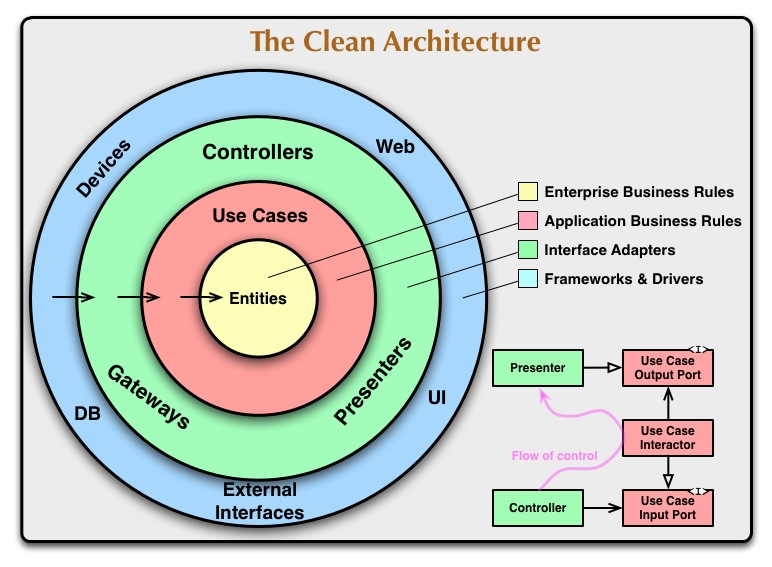
\includegraphics[width=0.85\textwidth]{Images/Arch/clean.png}
    \caption{Clean Architecture (Uncle Bob)}
    \label{fig:clean-arch}
\end{figure}

Mặc dù ma trận chấm điểm chỉ ra sự phù hợp có thể so sánh giữa kiến trúc Microservices (4.15) và Layered (4.00), các ràng buộc thực tế ủng hộ thiết kế phân lớp. Tuy nhiên, kiến trúc phân lớp truyền thống gặp phải vấn đề kết hợp chặt chẽ giữa các lớp, trong đó các lớp trên phụ thuộc trực tiếp vào các triển khai lớp dưới. Sự kết hợp này cản trở khả năng kiểm thử và làm cho việc thay thế công nghệ trở nên khó khăn \cite{martin2017}.

Clean Architecture, được đề xuất bởi Robert C. Martin, giải quyết những hạn chế này thông qua \textit{đảo ngược phụ thuộc} \cite{martin2017}. Thay vì cho phép các lớp bên ngoài phụ thuộc trực tiếp vào các triển khai bên trong, Clean Architecture yêu cầu tất cả các phụ thuộc hướng vào trong về phía logic nghiệp vụ (entities và use cases). 
Các mối quan tâm về cơ sở hạ tầng—cơ sở dữ liệu, framework, công nghệ, UI trở thành các plugin triển khai các giao diện được xác định bởi miền cốt lõi.

\subsubsection*{a. Các tầng chính}
\begin{table}[h]
\centering
\begin{tabular}{>{\bfseries}p{4.5cm}p{4cm}p{4.5cm}}
\toprule
\textbf{Tầng} & \textbf{Thành phần chính} & \textbf{Vai trò} \\
\midrule
UI / Interface Layer & Controller, Presenter, ViewModel, View & Tiếp nhận và hiển thị dữ liệu với người dùng. \\
\addlinespace
Application Layer & UseCase Interactor, InputBoundary, OutputBoundary & Chứa logic nghiệp vụ ứng dụng (use case). \\
\addlinespace
Domain Layer & Entities & Chứa logic nghiệp vụ cốt lõi, không phụ thuộc framework. \\
\addlinespace
Infrastructure Layer & DataAccessInterface, DataAccess, Database & Thao tác lưu trữ dữ liệu (DB, API, file...). \\
\bottomrule
\end{tabular}
\end{table}

\begin{figure}[h]
\centering
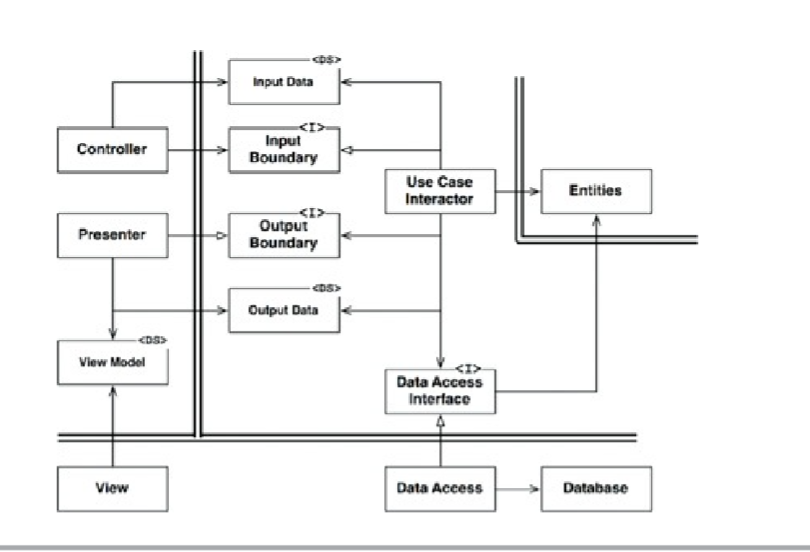
\includegraphics[height=0.5\textwidth]{Images/Arch/clean_flow.png}
\caption{A typical scenario for a system utilizing a database follow Clean Architecture}
\label{fig:clean_full}
\end{figure}

\subsubsection*{b. Luồng hoạt động chi tiết (Clean Architecture Flow)}
\textbf{Bước 1 -- Controller nhận input từ người dùng}\\
Người dùng gửi request (qua web form, API, hay giao diện). \textbf{Controller} nhận dữ liệu đầu vào (\textit{Input Data}) và gói lại trong một \textbf{Data Transfer Object (DTO)} -- ví dụ \texttt{CreateOrderRequest} hoặc \texttt{LoginRequest}. Controller không xử lý nghiệp vụ mà chuyển tiếp qua interface \texttt{InputBoundary}.
\vspace{0.3cm}

\textbf{Bước 2 -- InputBoundary chuyển dữ liệu vào Use Case}\\
\texttt{InputBoundary} là một \textbf{interface}, đảm bảo Controller không phụ thuộc trực tiếp vào logic nghiệp vụ. \texttt{UseCaseInteractor} implement \texttt{InputBoundary}, nên khi Controller gọi interface này, luồng điều khiển vào bên trong \textbf{Application Layer}.
\vspace{0.3cm}

\textbf{Bước 3 -- Use Case Interactor thực thi nghiệp vụ}\\
Đây là trái tim của ứng dụng (\textit{application business rules}). \texttt{UseCaseInteractor}:\\
-- Gọi \textbf{Entities} để áp dụng logic nghiệp vụ (ví dụ: tính tổng tiền, kiểm tra điều kiện).\\
-- Dùng \texttt{DataAccessInterface} để lấy dữ liệu thật từ DB (thông qua repository).\\
-- Kết quả xử lý được đóng gói lại thành \texttt{OutputData} (cũng là DTO).
\vspace{0.3cm}

\textbf{Bước 4 -- OutputBoundary trả kết quả ra ngoài}\\
Sau khi xử lý xong, \texttt{UseCaseInteractor} gửi \texttt{OutputData} qua \texttt{OutputBoundary} (interface). \textbf{Presenter} implement \texttt{OutputBoundary}, nên sẽ nhận được dữ liệu này.
\vspace{0.3cm}

\textbf{Bước 5 -- Presenter chuyển đổi dữ liệu cho UI}\\
Presenter không xử lý nghiệp vụ mà chỉ lo định dạng dữ liệu để hiển thị:\\
-- Chuyển Date thành chuỗi ``31/10/2025'', Currency thành ``1,000 VND''.\\
-- Đưa các cờ (flags) như ``button enabled'', ``menu visible'' vào \textbf{ViewModel}.

ViewModel là một Data Transfer Object (DTO) chứa dữ liệu UI-friendly.
\vspace{0.3cm}

\textbf{Bước 6 -- View hiển thị dữ liệu cho người dùng}\\
\textbf{View} chỉ cần nhận ViewModel và render ra giao diện (HTML, React component, XML layout, ...). View không chứa logic nghiệp vụ, chỉ hiển thị đúng dữ liệu đã được Presenter chuẩn bị.

\subsubsection*{c. Cải tiến kiến trúc này mang lại một số lợi thế phù hợp với yêu cầu dự án:}

\textbf{Khả năng kiểm thử nâng cao.} Các lớp logic nghiệp vụ hoàn toàn độc lập với cơ sở hạ tầng. Các bài kiểm thử đơn vị xác minh các use case mà không yêu cầu kết nối cơ sở dữ liệu hoặc framework UI, cải thiện đáng kể tốc độ thực thi kiểm thử và độ tin cậy.

\textbf{Độc lập công nghệ.} Miền cốt lõi xác định các hợp đồng (giao diện) thay vì phụ thuộc vào các công nghệ cụ thể. Thay thế PostgreSQL bằng MongoDB, hoặc chuyển từ NestJS sang Spring Boot, chỉ yêu cầu các triển khai adapter mới mà không sửa đổi các quy tắc nghiệp vụ.

\textbf{Không phụ thuộc framework.} Không giống như các framework MVC truyền thống kết hợp chặt chẽ code ứng dụng với các lớp framework, Clean Architecture cô lập các phụ thuộc framework tại các ranh giới hệ thống. Sự độc lập này giảm khóa nhà cung cấp và tạo điều kiện nâng cấp framework.

\textbf{Ranh giới module rõ ràng.} Kiến trúc xác định rõ ràng bốn lớp khái niệm: Entities (mô hình miền), Use Cases (quy tắc nghiệp vụ ứng dụng), Interface Adapters (controllers, presenters, gateways) và Frameworks \& Drivers (công cụ bên ngoài). Các ranh giới này phù hợp với các mẫu cộng tác nhóm, trong đó các thành viên khác nhau có thể làm việc trên các lớp khác nhau với xung đột tối thiểu.

\subsubsection{Quyết định kiến trúc}

Dựa trên đánh giá định lượng và phân tích định tính, chọn \textbf{Clean Architecture} làm phong cách kiến trúc chính, với tích hợp có chọn lọc các \textbf{mẫu Event-Driven} cho các hệ thống con thời gian thực. Quyết định này được biện minh thông qua lý do sau:

\textbf{Phù hợp với ràng buộc dự án.} Sự tách biệt lớp rõ ràng của Clean Architecture hỗ trợ cấu trúc nhóm ba người bằng cách thiết lập quyền sở hữu module rõ ràng và giảm xung đột merge. Sự nhấn mạnh của kiến trúc vào khả năng kiểm thử đáp ứng yêu cầu học thuật về chất lượng code và tài liệu có thể chứng minh \cite{martin2017}.

\textbf{Độ phức tạp cân bằng.} Trong khi microservices cung cấp khả năng mở rộng vượt trội, chúng yêu cầu chuyên môn về hệ thống phân tán và cơ sở hạ tầng DevOps vượt quá tài nguyên dự án. Clean Architecture cung cấp 80\% lợi ích về khả năng bảo trì và mở rộng với 40\% độ phức tạp triển khai, đại diện cho tỷ lệ nỗ lực-lợi ích tối ưu \cite{richards2020}.

\textbf{Giá trị giáo dục.} Kiến trúc thể hiện rõ ràng các nguyên tắc kỹ thuật phần mềm: tách biệt các mối quan tâm, đảo ngược phụ thuộc, tách biệt giao diện và trách nhiệm đơn lẻ. Những lợi ích sư phạm này phù hợp với các mục tiêu học tập của dự án học thuật.

\textbf{Đáp ứng tăng trưởng.} Mặc dù ban đầu triển khai ở quy mô nhỏ (50 xe, 150 người dùng), bản chất module hóa của Clean Architecture hỗ trợ thêm tính năng gia tăng—các công cụ khuyến nghị AI, phân tích nâng cao, tích hợp bên thứ ba—mà không cần tái cấu trúc kiến trúc. Lớp use case có thể mở rộng với các yêu cầu nghiệp vụ mới trong khi duy trì các định nghĩa entity ổn định.

\textbf{Chiến lược công nghệ.} Các mẫu hướng sự kiện bổ sung cho Clean Architecture cho các yêu cầu cụ thể: cập nhật vị trí thời gian thực (qua WebSocket), gửi thông báo (qua hàng đợi thông điệp) và thu thập dữ liệu phân tích (qua streaming sự kiện). Những mẫu chiến thuật này tích hợp như các adapter trong framework Clean Architecture thay vì quyết định cấu trúc hệ thống tổng thể.

Quyết định kiến trúc thừa nhận các đánh đổi: Clean Architecture đưa ra nhiều code boilerplate ban đầu hơn so với các framework monolithic và đảo ngược phụ thuộc yêu cầu tuân thủ kỷ luật các hợp đồng giao diện. Tuy nhiên, những chi phí này đại diện cho các khoản đầu tư trả trước mang lại lợi ích khả năng bảo trì dài hạn—một sự trao đổi đáng giá cho một hệ thống dự định chứng minh các thực hành phát triển phần mềm chuyên nghiệp.